\begin{frame}[fragile]{Proposed Method} 
\vspace{0.3cm}

\begin{center}
\begin{tikzpicture}[scale=0.55, every node/.style={scale=0.55}, node distance = 2cm, auto]
   
  \node [outer sep=0cm] (environment) at (0,0)  {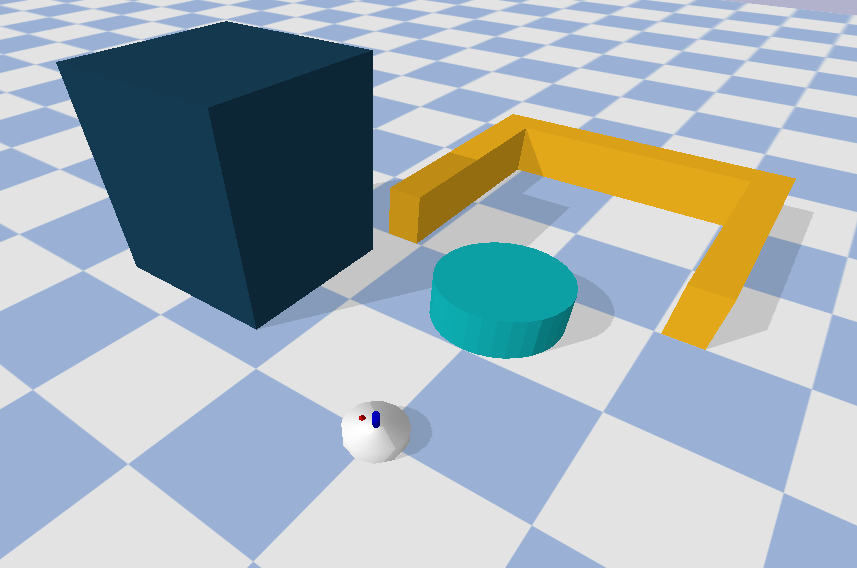
\includegraphics[width=4.6cm]{figures/introduction/blockade}}; 

  \draw [myEvenLighterColor,
  rounded corners=0.3cm, 
  line width=0.3cm]  
  (environment.north west) -- 
  (environment.north east) --
  (environment.south east) --
  (environment.south west) -- cycle  ;

  \node [block,
  above of=environment,
  minimum height=2cm,
  minimum width=5cm,
  node distance=4.1cm,
  outer sep=0cm] (hgraph) {Hypothesis Algorithm};

  \node [block, 
  above of=hgraph, 
  node distance=3.3cm, 
  minimum width=5cm,
  minimum height=2.0cm] (kgraph) {Knowledge Graph};
    
  % Draw edges
  \draw[-stealth] ([yshift=0.155cm, xshift=0.4 cm]environment.north) -- node [xshift=-.05cm, right] {\shortstack[]{sensor\\measurements}}([xshift=0.4 cm]hgraph.south) ;
  \draw[-stealth] ([xshift=-0.4 cm]hgraph.south) -- node [left] {robot input}([yshift=0.155cm, xshift=-0.4 cm]environment.north) ;
  \draw[stealth-] (hgraph.west) -- node [above] {task} ++(-1, 0);


  \draw[-stealth] ([xshift=-0.4cm]kgraph.south) -- node [left] {\shortstack[]{action\\suggestions}}([xshift= -0.4cm]hgraph.north) ;
  \draw[stealth-] ([xshift=0.4cm]kgraph.south) -- node [right] {\shortstack[]{action\\feedback}}([xshift= 0.4cm]hgraph.north) ;
\end{tikzpicture}
\end{center}

\end{frame}
